%! TEX root = ../../super_nova_2024.tex
\documentclass[../../super_nova_2024]{subfiles}

% ローカル下書き用
% \documentclass{supernova_pre}
% このクラスの中に大体のパッケージは入ってるので基本何でもかけるはず
% 追加したいパッケージがあればここに記入


\begin{document}

\chapter{彗星撮影にチャレンジ!} % タイトル
\rightline{M1 森山 陽介} % 学年と名前(ハンドルネームでも可)

\begin{figure}
  \centering
  \includegraphics[width=\textwidth]{img/DSC_2704.jpg}
  \caption{2024年10月15日屋上天文台での紫金山・アトラス彗星観測会の様子。中央にある望遠鏡は筆者の私物であり、本稿の影の主役であったりする。}
\end{figure}
\section{最近彗星がアツい!}

2024年10月12日、C/2023 A3 (Tsuchinshan-ATLAS)と命名された彗星「紫金山・アトラス彗星」が地球に再接近$^\text{\cite{nao_C2023A3}}$、東京調布の夕空にも堂々たる長い尾を持った姿を現しました。

天文部員として活動をはじめて4年目、望遠鏡と赤道儀を使った星雲・星団の撮影に挑戦していますが、去年から今年にかけては明るい彗星も頻繁に到来するチャンスの年でした。本稿では、彗星について基本事項をおさらいした上で、観測・撮影に挑戦したZTF彗星 (C/2022 E3 (ZTF))、ポンス・ブルックス彗星 (12P/Pons-Brooks)、紫金山・アトラス彗星 (C/2023 A3 (Tsuchinshan-ATLAS))についてお伝えします。

\section{彗星について}

まず最初に、彗星についておさらしいましょう$^\text{\cite{nao_comet}}$。彗星は惑星や準惑星、小惑星と並ぶ太陽系を構成する天体です。
構成成分の8割を占める水と、二酸化炭素、一酸化炭素やその他のガスと微量の塵から成る氷の塊で、よく「砂で汚れた雪玉」と表現されます。太陽に近づいたときにその熱で本体から融けたガスや塵が輝くことで「コマ」と呼ばれる淡い光が本体を包むように形成されます。また、彗星は「ほうき星」とも呼ばれるように、長い尾を引く姿でも有名です。融けたガスと塵によって2種類の尾が作られます$^\text{\cite{canon_comet}}$。ひとつは、太陽紫外線を受けてイオンと電子に電離したガスが太陽風を受けて作る「イオンの尾」、もうひとつは、塵が太陽光の圧力「光圧」によって広がり太陽光を散乱して作る「ダストの尾」です。
この塵の一部は、彗星の軌道を周回し続け、その軌道に地球がぶつかる時に流星群として観測されます。先月のオリオン座流星群の母天体はあのハレー彗星 (1P/Halley)です。

黄道面と呼ばれる平面に沿ってほぼ円形の楕円軌道で公転する惑星と違い、彗星の軌道は細長い楕円軌道や放物線・双曲線軌道を描きます。放物線・双曲線軌道のように一度だけ太陽に近づき二度と戻ってこない彗星や、楕円軌道ではあるものの公転周期が200年より長い彗星は「長周期彗星」と呼ばれ、200年以内の彗星は「短周期彗星」と呼ばれています。彗星などの天体は、発見されてから仮符号がつけられます。彗星ではCometを表す``C/''が接頭語として付加されます。この中で、短周期彗星もしくは2回以上の近日点を持つ長周期彗星と判明した場合には``P/''の接頭語になります。また、消滅した彗星には``D/''が、短期間の観測で不確定な彗星には``X/''が振られます。この接頭語に続いて、「発見された年」と「発見された月を示すアルファベット」 (\tabref{alphabet})、「期間内の発見順の番号」が続きます。また、この後ろには括弧書きで発見者・観測プロジェクトの名前が表記されます$^\text{\cite{nao_prov-comet}}$。
先月地球に接近した紫金山・アトラス彗星は``C/2023 A3 (Tsuchinshan-ATLAS)''という符号が振られており、「2023年1月前半の3番目に紫金山天文台とATLASシステムによって発見された彗星」ということになります。

\begin{table}
  \small
    \centering
    \caption{発見された月を示すアルファベットの対照表。Iを除くA--Yのアルファベットが各月の前半後半それぞれに順に対応している。}
    \label{tab:alphabet}
    \begin{tabular}{c|cccccccccccc}\hline
        月 & 1月 & 2月 & 3月 & 4月 & 5月 & 6月 & 7月 & 8月 & 9月 & 10月 & 11月 & 12月 \\
        \hline
        前半(1--15日) & A & C & E & G & J & L & N & P & R & T & V & X \\
        後半(16日--) & B & D & F & H & K & M & O & Q & S & U & W & Y \\
        \hline
    \end{tabular}
\end{table}


\section{ZTF彗星 (C/2022 E3 (ZTF))}

私が天文部に入ってから初めて観測した彗星はZTF彗星でした。2022年3月2日にアメリカのZwicky Transient Facility (ZTF)による観測で発見され、近日点は2023年1月13日、2023年2月2日に近地点を迎えました。SNSでこの彗星の接近を知った当時学域3年生の私たちは、2023年2月1日から2日にかけての晩にいつもの神代植物公園自由広場に集まり観測を試みました。明るい惑星や、いつも同じ場所にいるメシエ天体などとは異なり、彗星は暗く日によって大きく移動するため、前日からの予習が効きません。そこで当日手動で望遠鏡と赤道儀を使って探し出すのは難しいだろうと、ひとまずカメラと望遠レンズと三脚だけで存在だけでも確認しようとしました。当日のZTF彗星は、ぎょしゃ座の一等星カペラと北斗七星の柄杓の先端にあるドゥーべ、北極星ポラリスを結んだ三角形の内心のような位置(カペラ寄り)に見つけることができました。\figref{ZTF}は当時撮影した一枚です。画像中央にボヤッとした星が写っているのがわかると思います。これがZTF彗星です。

\begin{figure}
    \centering
    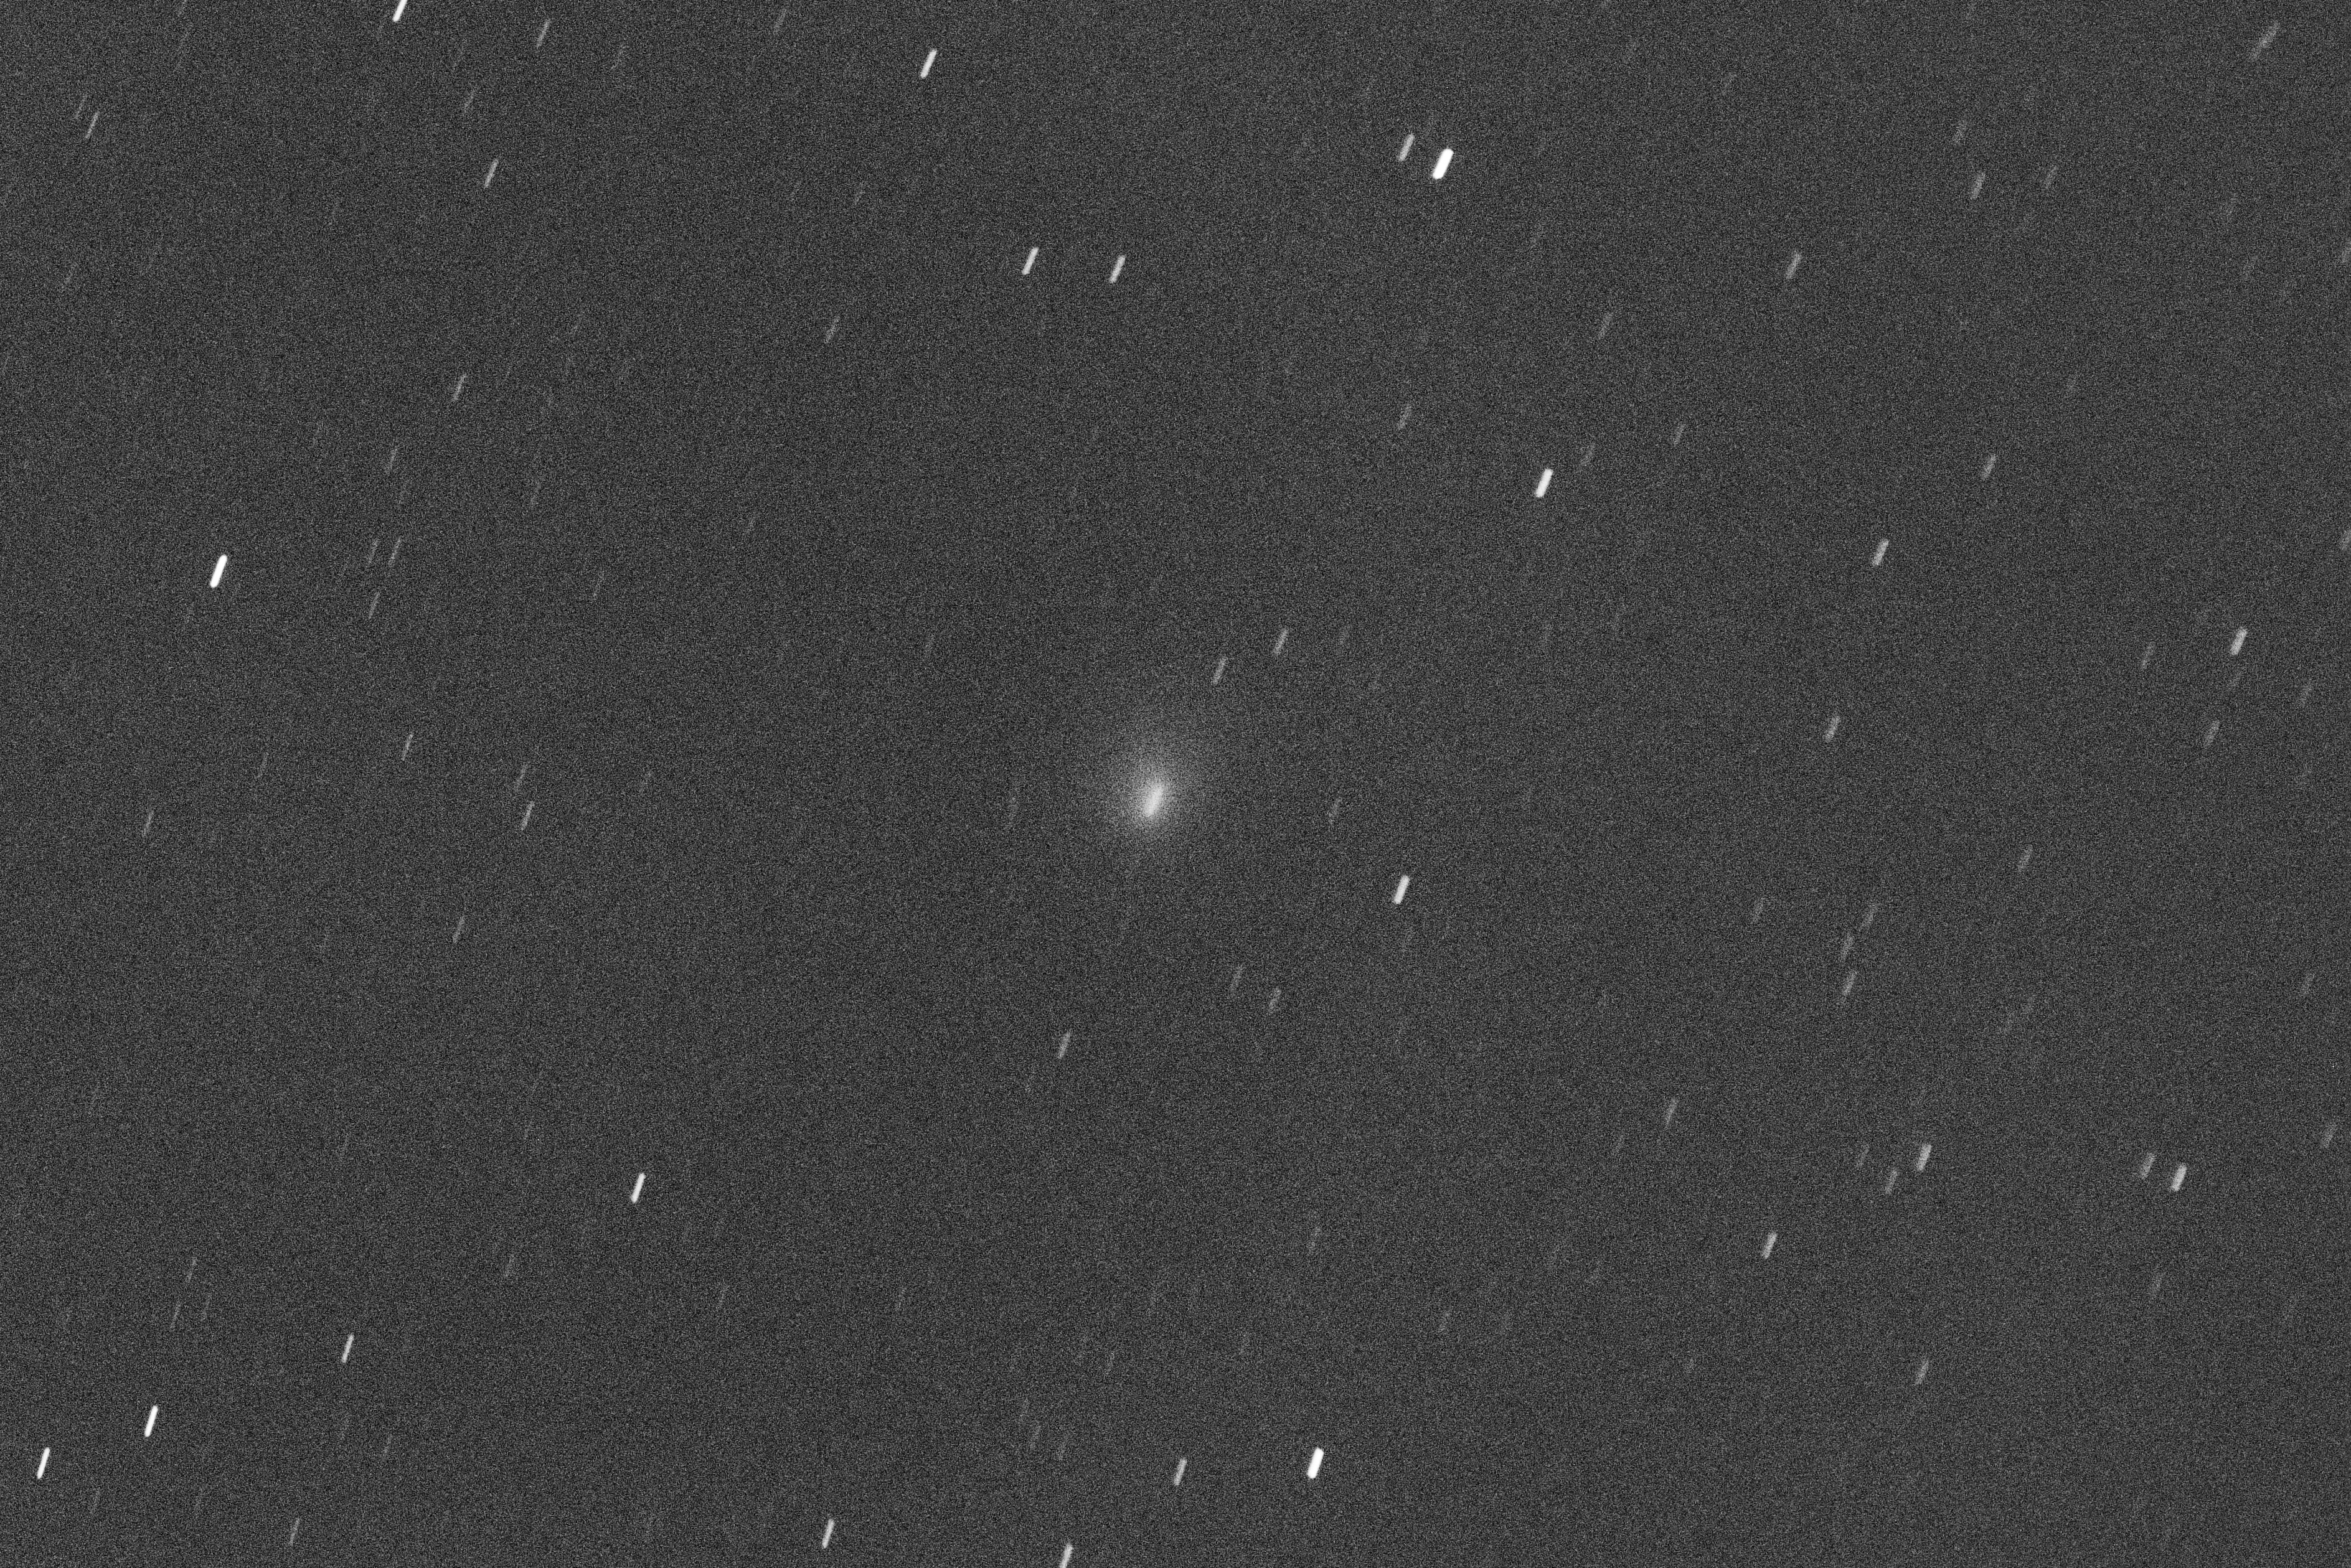
\includegraphics[width=.8\columnwidth]{img/ZTF_unstacked.jpg}
    \caption{2023年2月2日午前0時2分頃に撮影されたZTF彗星。中央にぼんやりと広がるコマが確認できる。}
    \label{fig:ZTF}
\end{figure}


\section{ポンス・ブルックス彗星 (12P/Pons-Brooks)}

ZTF彗星の観測後、2023年9月には西村彗星が太陽に接近$^\text{\cite{nao_Nishimura}}$が話題となりましたが、観測条件が厳しく観測には至れなかったりと、密かに彗星観測・撮影への関心が高まっていました。そんな中、2024年の秋に大彗星と噂される紫金山・アトラス彗星が到来すると知り、彗星撮影に向けて準備を始めました。彗星撮影に向けてはカメラに加えて次の5つの要素が必要になります。
\begin{itemize}
    \item 望遠鏡
    \item 赤道儀と三脚
    \item 赤道儀を自動導入化するモーターとドライバー
    \item PC(彗星の位置などを入力するためのプラネタリウムソフト)
    \item Comet Band Passフィルター(彗星の放つ波長帯を通し都市光害をカット・軽減する)
\end{itemize}
これらが一通り揃ってきた2024年の初めごろ、秋の大彗星に向けた前哨戦としてちょうどいいタイミングで、ポンス・ブルックス彗星 (12P/Pons-Brooks)が地球に接近していました。

ポンス・ブルックス彗星は1812年にフランスのポンス氏、1883年にブルックス氏によって発見された公転周期70年の短周期彗星です$^\text{\cite{astroarts_12P}}$。2024年の回帰では、2024年4月21日に太陽に最接近し、4等級まで明るくなるとされていました。当時私たちは学域4年、一通り卒業論文や発表から解放された一同は、このポンス・ブルックス彗星を観測するため、卒業旅行も兼ねて伊豆半島2泊3日の遠征を敢行しました。この遠征では天候に恵まれず観測には至りませんでしたが、調布に戻ってから2024年3月20日から22日にかけて西の空が晴れたため、観測に踏み切りました。(\figref{Pons_Obs})

\begin{figure}
    \centering
    \includegraphics[width=.8\columnwidth]{img/12P_shooting_image.JPG}
    \caption{2024年3月22日の観測風景。ドーム内に三脚・赤道儀を組み、西の空に望遠鏡を向けている。導入を制御したPCには、彗星が写っている。}
    \label{fig:Pons_Obs}
\end{figure}

撮影にあたっては、3年の夏に購入したVixen AP赤道儀、4年の夏に購入した望遠鏡を使っています。AP赤道儀は2軸モーター仕様に、Vixen Wireless Unitを導入して自動導入仕様に仕上げています。彗星撮影に合わせて、彗星の波長を通しつつ、光害をカットするCBPフィルタを導入しています。彗星の導入にはPCをWireless Unitに接続し、フリーの天体撮影統合ソフト``N.I.N.A''から目標の彗星の座標を入力して、自動導入を行なっています。赤道儀によって、日周運動の追尾をしているため、通常の恒星は長時間露光でも流れて写ることはありませんが、彗星は微妙に日周運動とはずれているため、長時間露光しすぎると流れて写ってしまいます。そのため、20秒程度の短時間露光に抑えています。\figref{Pons-Brooks}は2024年3月22日に撮影したポンス・ブルックス彗星 (12P/Pons-Brooks)です。
左下に明るく写っているのが、彗星本体の核とコマと呼ばれるものです。誌面においてどのように見えているか不安ですが、左下から右上にかけて非常に淡くですが、尾の様子も確認できます。カメラで撮影し、その場で簡易な強調処理を行うことでようやく見えたこの彗星は、肉眼では双眼鏡を用いてもなかなか見ることができませんでした。また夕暮れどきの周囲の基準星も少ない時刻に導入を行い短時間で作業をしなければならない彗星撮影は、これまでの天体撮影とはまた一味違う苦労と楽しさがありました。

\begin{figure}[H]
  \centering
  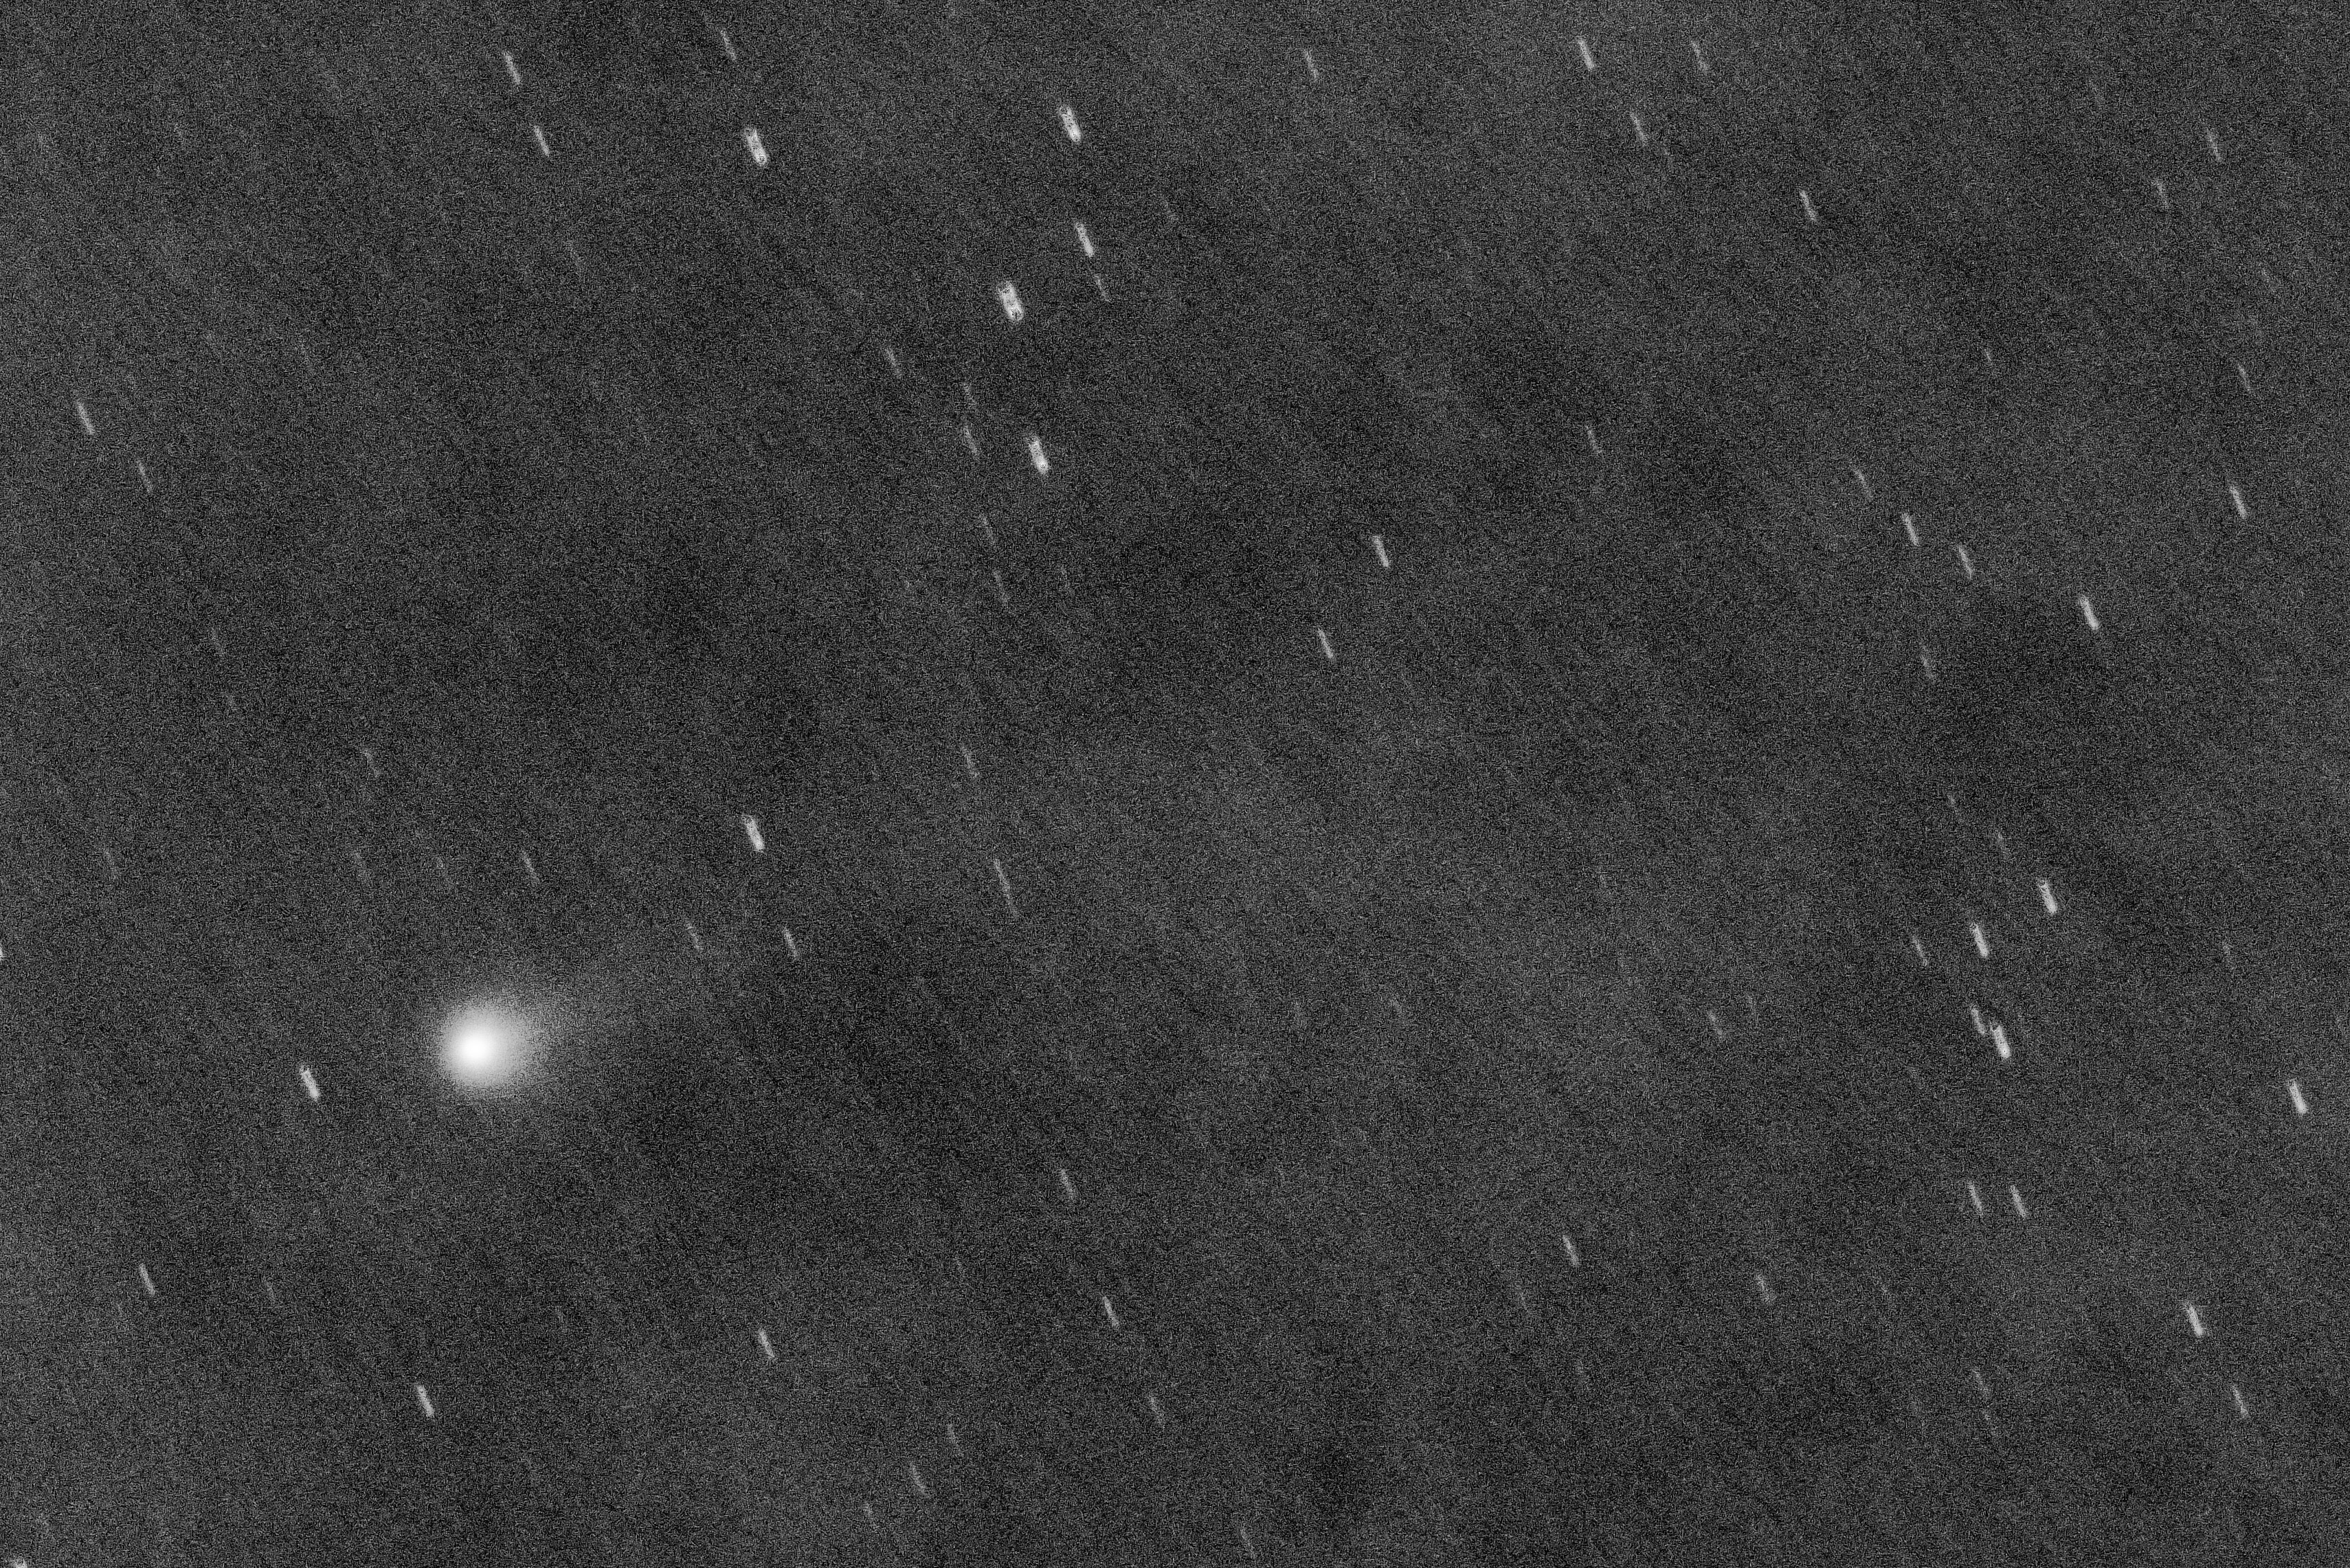
\includegraphics[width=.8\columnwidth]{img/12P-Pons-Brooks.jpg}
  \caption{2024年3月22日撮影のポンス・ブルックス彗星 (12P/Pons-Brooks)。彗星の動きに合わせてスタック処理をしているため、彗星以外の恒星が流れて写っている。}
  \label{fig:Pons-Brooks}
\end{figure}

\section{紫金山・アトラス彗星 (C/2023 A3 (Tsuchinshan-ATLAS))}

紫金山・アトラス彗星ことC/2023 A3 (Tsuchinshan-ATLAS)は、2023年1月9日に中国の紫金山 (拼音: z$\Grave{\textrm{{i}}}$ch$\Bar{\textrm{{i}}}$nsh$\Bar{\textrm{{a}}}$n; 英音: Tsuchinshan)天文台で発見された彗星です。その後観測されず、一時は観測報告が削除されたものの、地球に接近する小惑星を警戒するシステムATLASによって同年2月22日に再発見されました。そのため、二つの観測施設名を発見順に並べた「紫金山・アトラス彗星」と名付けられました。この彗星は、2024年9月28日に近日点を通過し、同年10月12日に地球に最接近しました。明るさを示す等級も楽観的に見積もって-3等級、悲観的に見積もっても3等級と非常に明るく、肉眼彗星\footnote{肉眼でも観察できるほど明るい彗星}として期待が集まっていました。軌道の都合上、近日点に向かう期間では南半球側で長い尾を引く姿が数多く撮影され、SNS上を賑やかしていました。当時まだ観測しにくい状態だった北半球側の我々は、「この写真は本当に同じ世界線のものなんだろうか」と指を咥えて見ることしかできませんでした。近地点となる10月12日より前の10月第1週の時期には、早朝の日の出までの時間が観測のチャンスとされていました。少しでも早くその姿を観たい一心で、我々M1\footnote{修士1年のこと}の有志は早起きしていつものように神代植物公園自由広場に集まり、観測を試みました。(\figref{1002}) しかし、生憎の天候で、日の出が近づくにつれて雲が集まり、観測することは叶いませんでした。一同一旦の帰路に着き、大学へ行く支度をしながらSNSを見ると、同じ日に八王子$^\text{\cite{HDV_blog}}$や横須賀$^\text{\cite{Hoshinavi}}$で撮影に成功したという報告があり、なんとももどかしい思いでした。


撮影に成功したのは、近地点を過ぎた10月13日でした。前日10月12日の観測会(\figref{1013})で、1人のM1部員が観測に成功したこともあってか、この日の観測会には多くの後輩たちも屋上天文台へ詰めかけました。\footnote{とはいっても、半数近くはM1なんですが…} 前日に撮影ができたとはいえ、空に浮かぶシミ程度だったため、さすがに肉眼で見えるまでにはならなかったかと思っていました\footnote{近日点に近づくまでの間に崩壊が始まっているという報告も上がっていたため}。しかし、日が暮れるにつれてカメラに収まりはじめ、双眼鏡で見え始め、終いには肉眼でもありありとその姿を見ることができました。\figref{Tsuchinshan-ATLAS}はこの日に屋上天文台から撮影した紫金山・アトラス彗星と電通大西2号館です。多くの彗星は前項のように、赤道儀とスタック処理が必要でしたが、今回は三脚に載せただけの1枚撮りでここまでその姿を映すことができました。誌面の都合上、モノクロとなっていますが、2024年調布祭の天文部教室展示では、部員それぞれが撮ったいろいろな彗星の写真が展示されていますので、是非カラーでその姿をお楽しみください。
\begin{figure}[H]
  \centering
  \begin{minipage}{0.49\columnwidth}
    \centering
    \includegraphics[width=\textwidth]{img/20241002_044541.jpg}
    \caption{2024年10月2日に紫金山・アトラス彗星の観測に挑戦するM1グループ。眠い目を擦りながら集まったが、同時に雲も集まり呆然と立ち尽くしている。}
    \label{fig:1002}
  \end{minipage}
  \begin{minipage}{0.49\columnwidth}
    \centering
    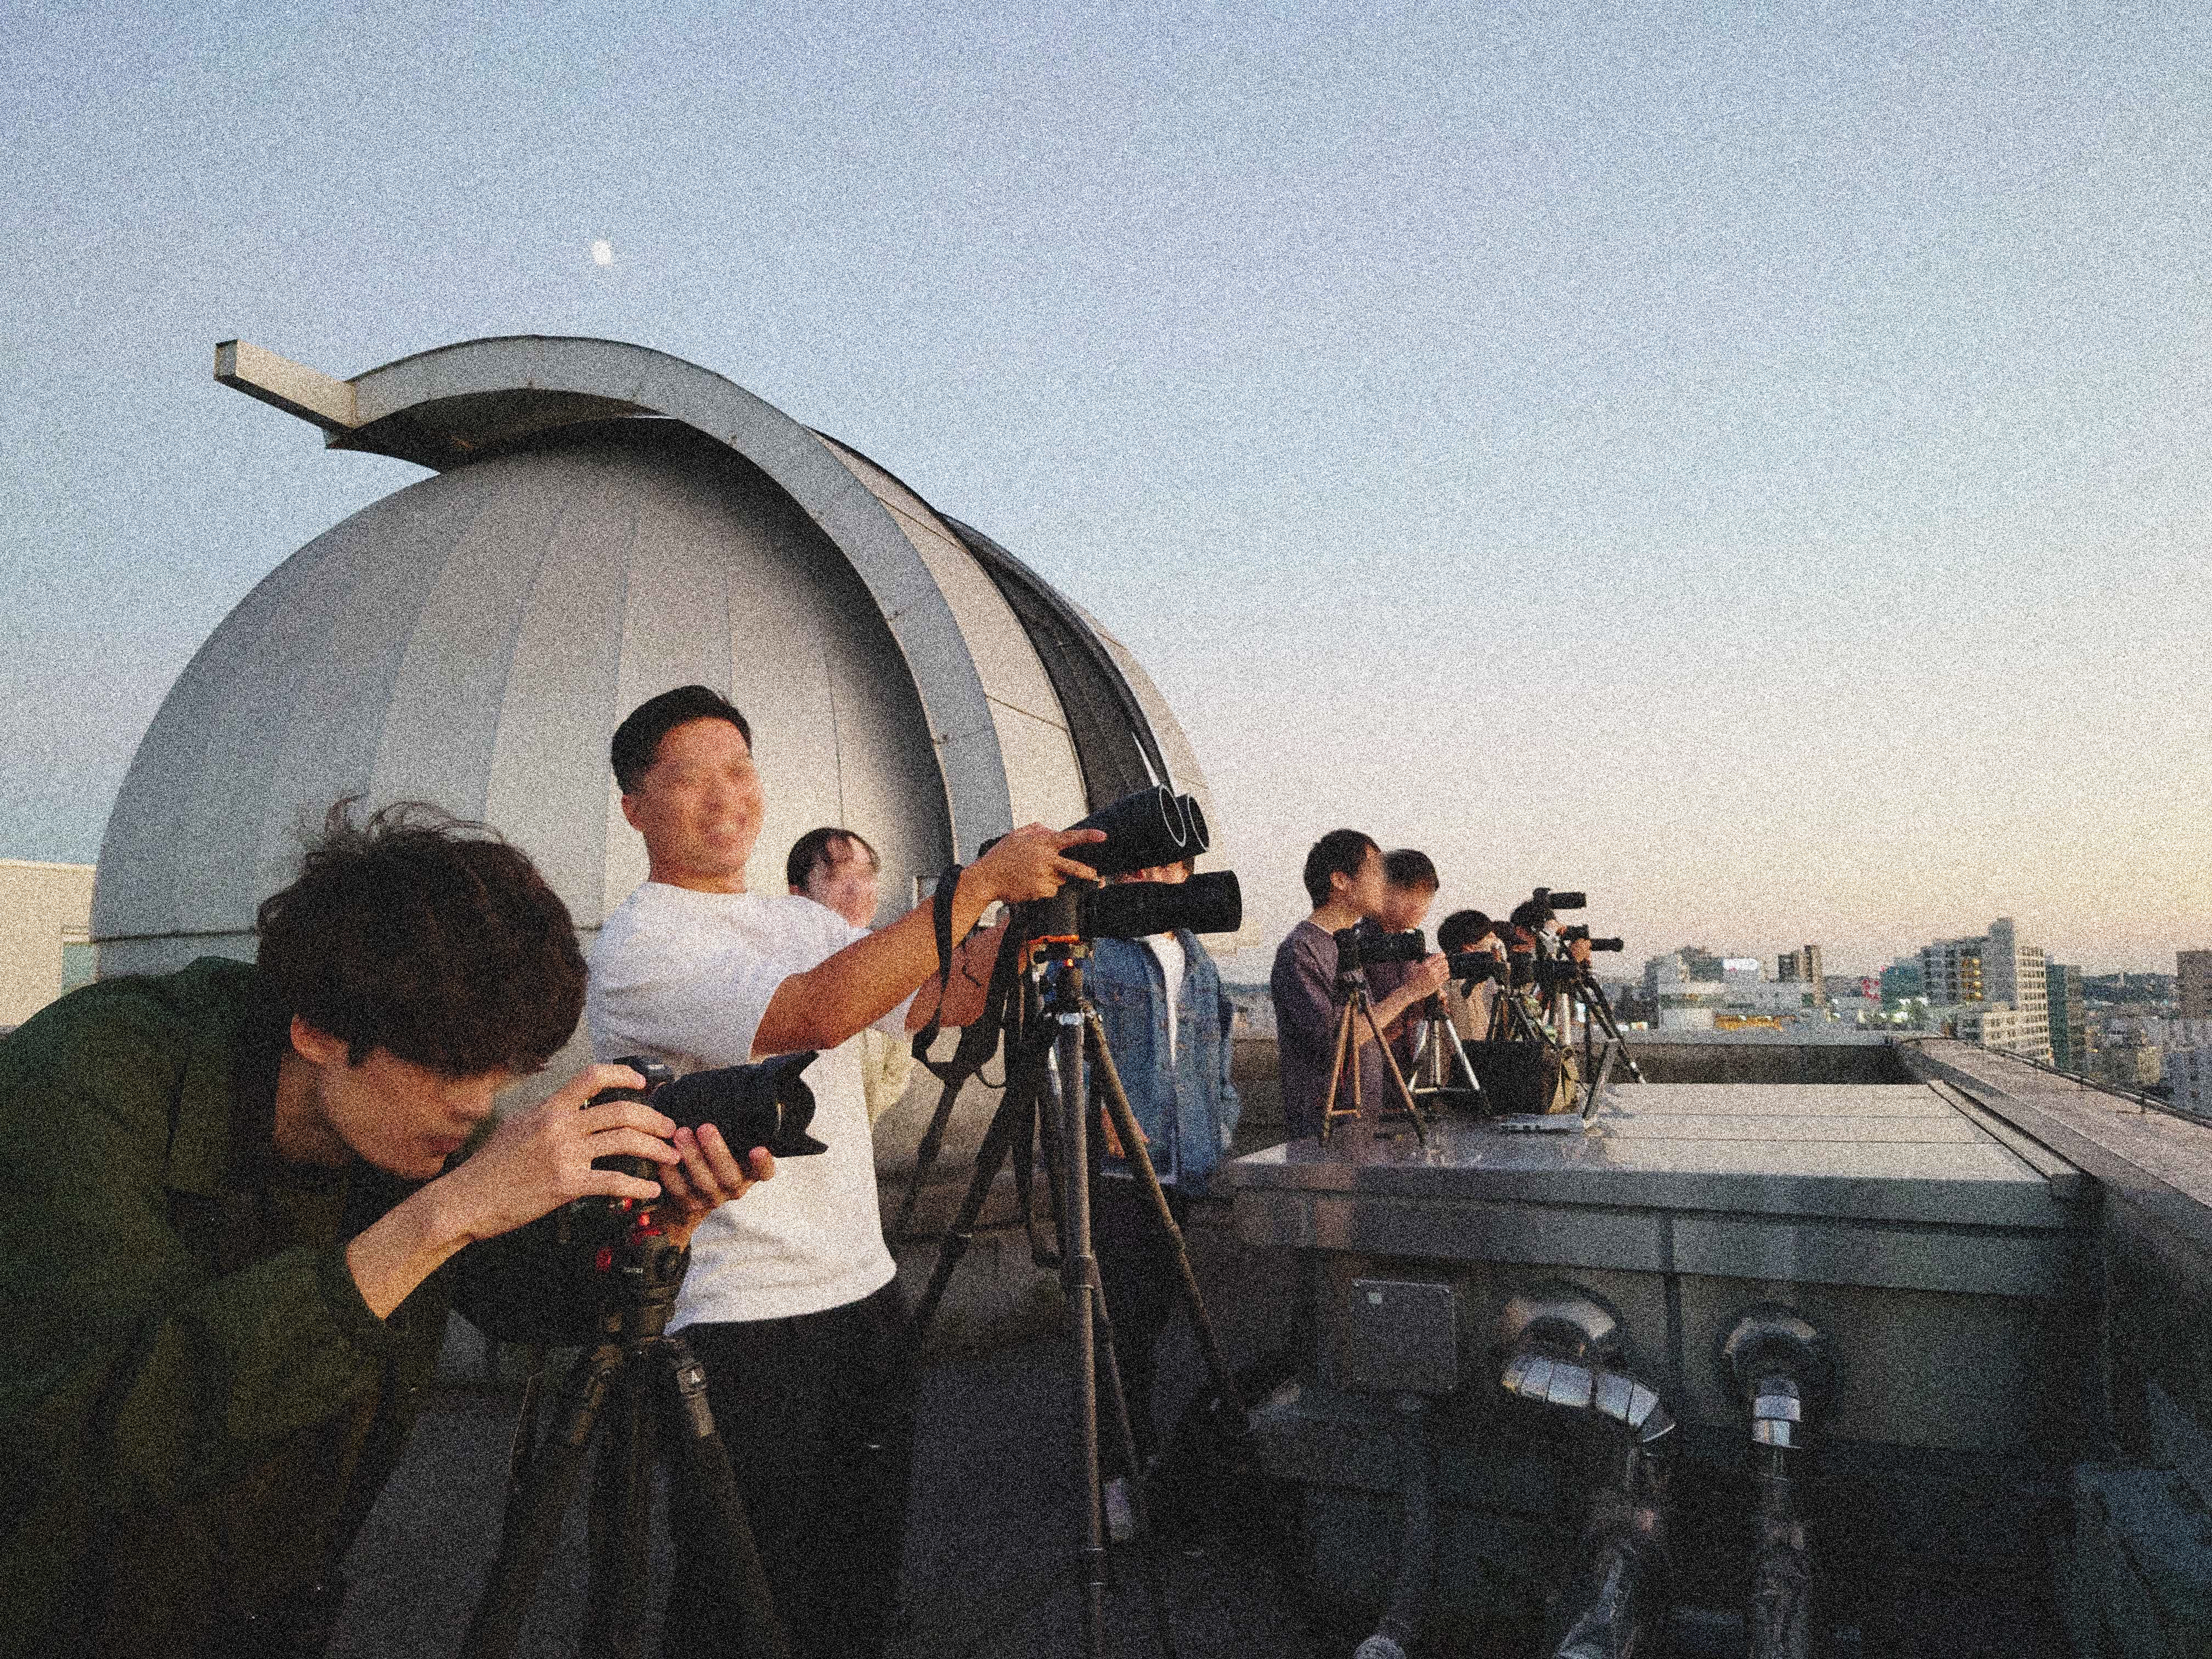
\includegraphics[width=\textwidth]{img/DSC_2673.jpg}
    \caption{2024年10月13日の紫金山・アトラス彗星観測会の様子。手前側に笑顔のM1集団、その奥には新進気鋭の後輩たちも彗星を狙ってカメラを構えている。}
    \label{fig:1013}
    \end{minipage}
\end{figure}

\begin{figure}
  \centering
  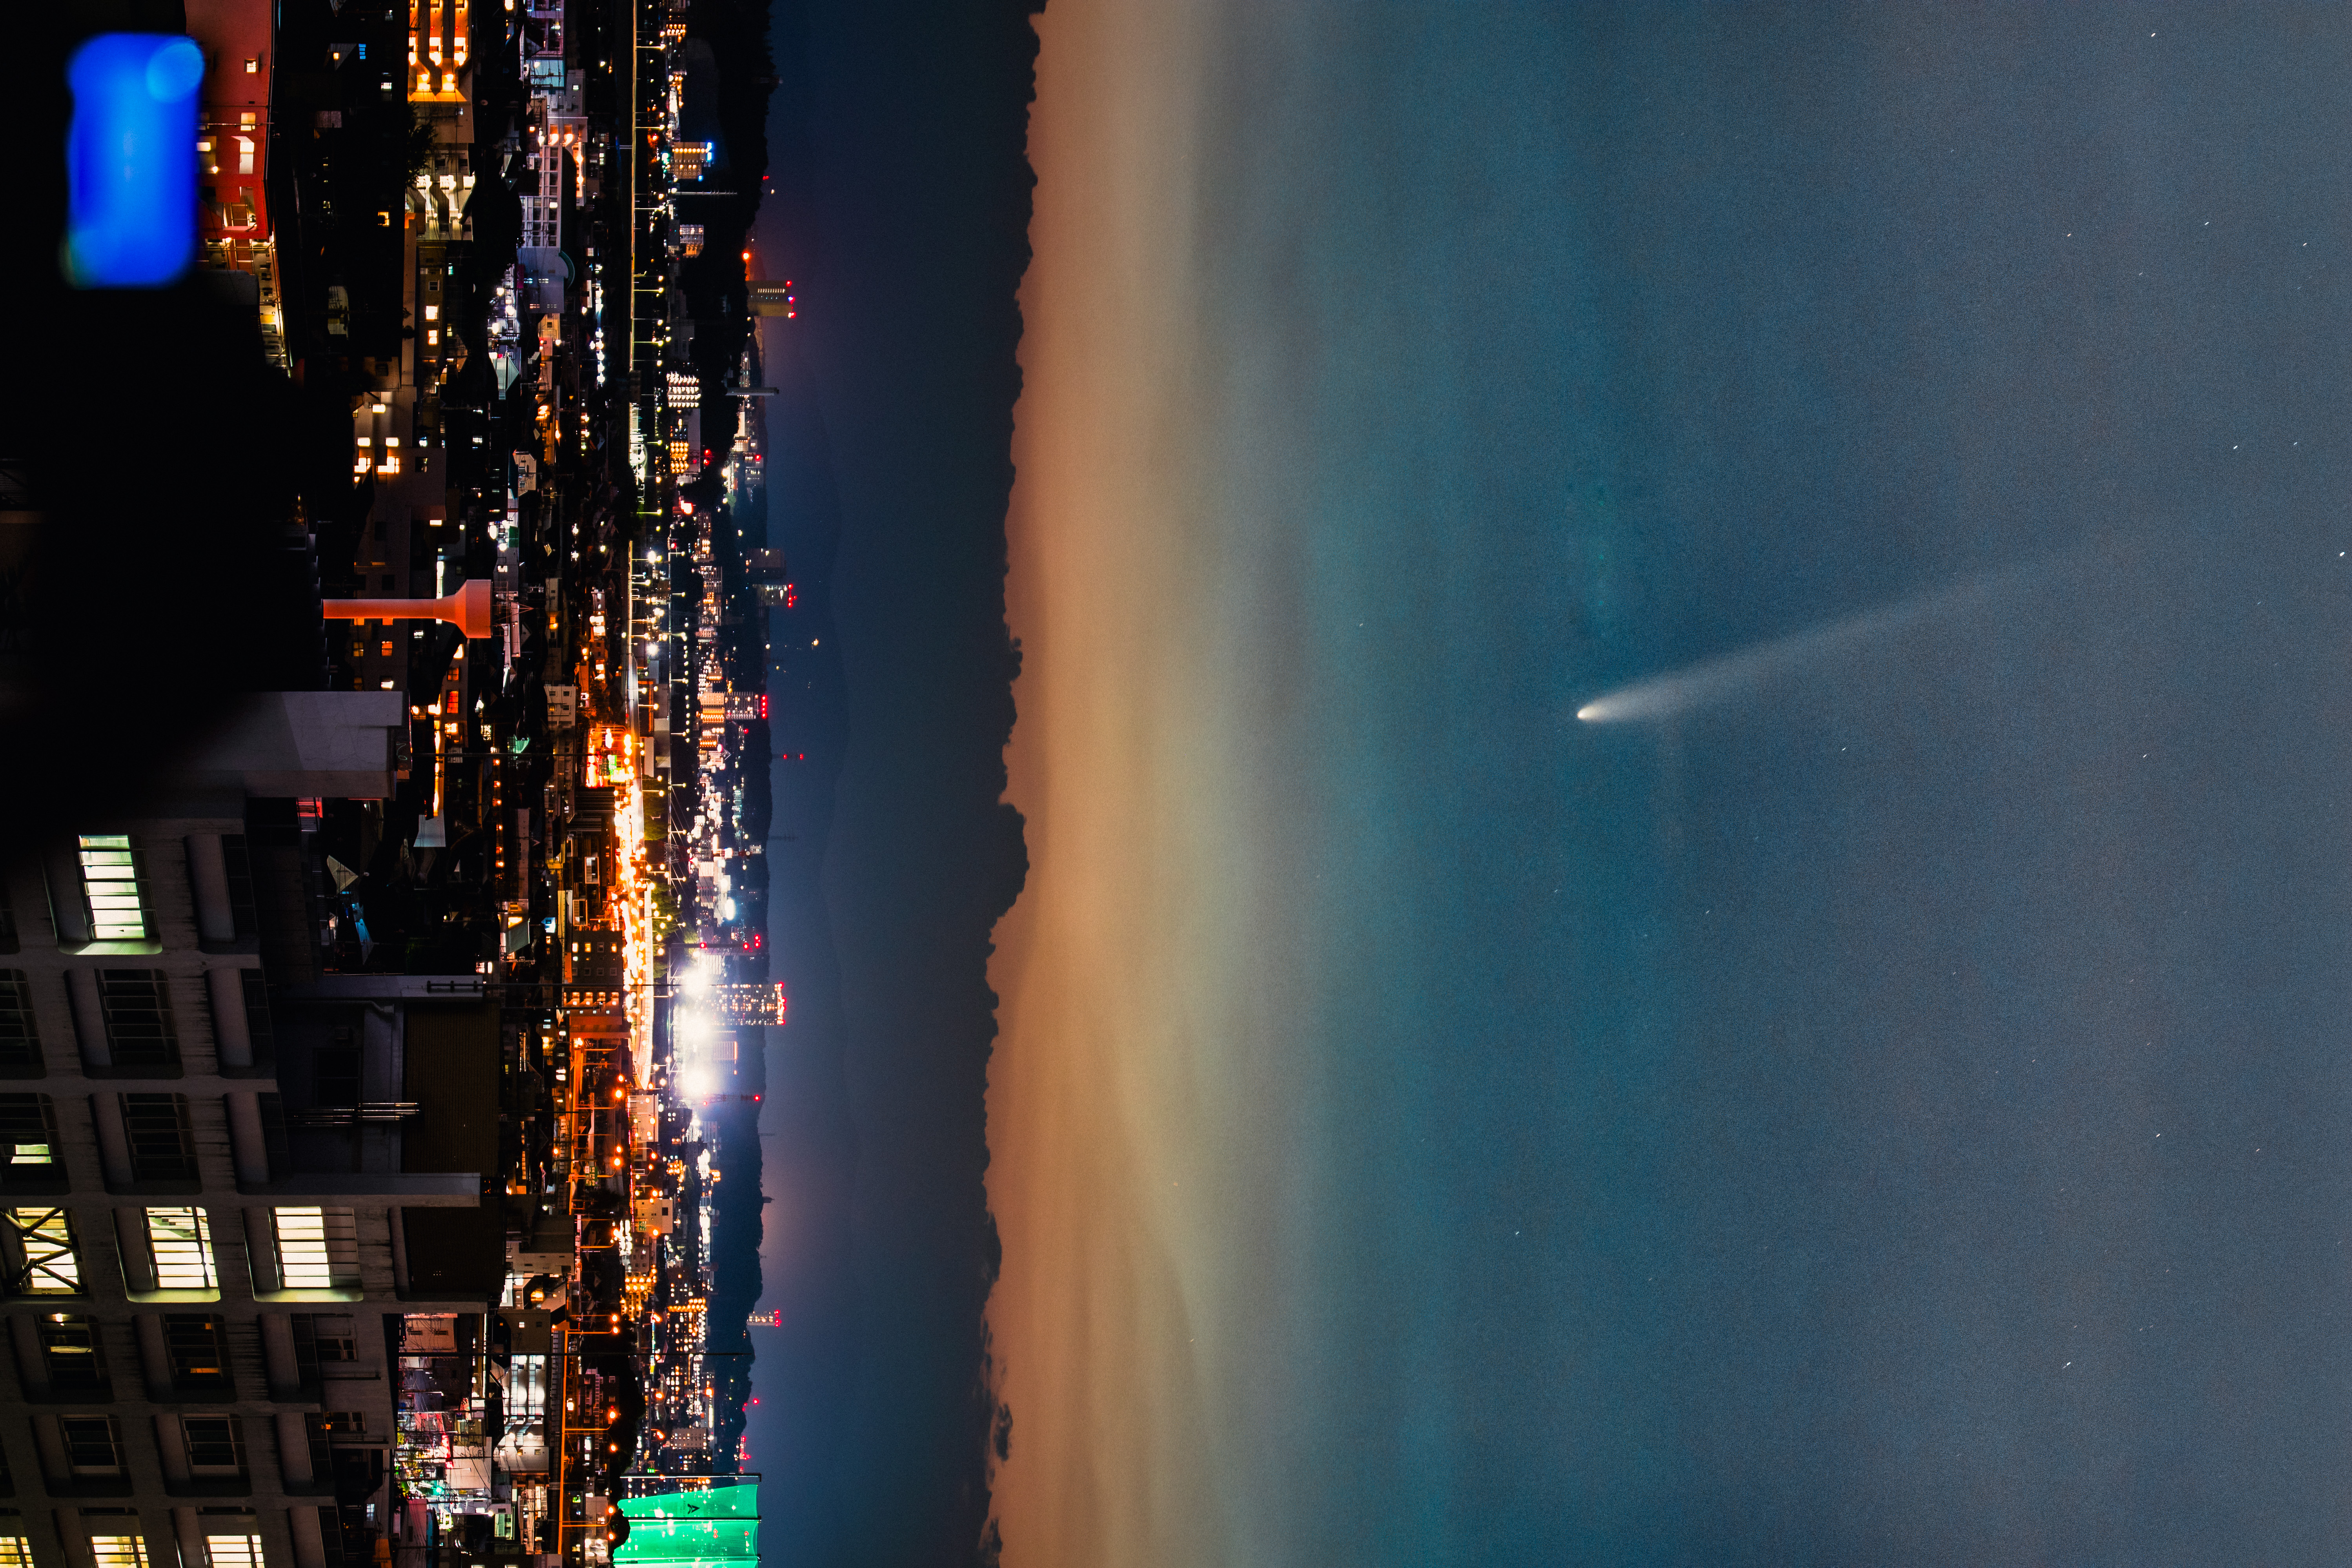
\includegraphics[width=\textwidth]{img/C_2023_A3_Siril.jpg}
  \caption{2024年10月13日に撮影したC/2023 A3 (Tsuchinshan-ATLAS)。 画面右下には電気通信大学 西2号館が写っている。中央地平線に
  3つ大きく光を放っているのは府中競馬場。その眩しい都市光害の中であってもなお大きく尾を引いた勇姿を魅せている。}
  \label{fig:Tsuchinshan-ATLAS}
\end{figure}

\clearpage
\section{さいごに}

撮り始めてみて、よく調べてみると、等級が低いだけで実は毎年多くの彗星が到来しているようです。しかし、今回の紫金山・アトラス彗星のように多くの人が目にするような彗星はレアな天体イベントです。
近地点を超え、日本でもその姿が肉眼で捉えられるようになるまでは、本当に肉眼彗星となるのかその予報を疑うこともありました。いざその姿を見ると、いつもの広場にも多くの人が集まり、その姿を一目見ようと挑戦していました。ほとんどの彗星は一度近づいたが最後、一期一会の出会いです。短周期のハレー彗星も次は2061年。一生に何度このチャンスがやってくるかわからない世紀の天体ショー、次いつ観られるかわからない儚さが、人々の心を惹きつけるのでしょうか?



\begin{thebibliography}{9}
    \bibitem{nao_C2023A3} 国立天文台, ほしぞら情報2024年10月, ``(解説)紫金山・アトラス彗星の観察チャンス(2024年10月)'', \url{https://www.nao.ac.jp/astro/sky/2024/10-topics05.html}
    \bibitem{nao_comet} 国立天文台, 彗星, ``彗星とはどのような天体か'', \url{https://www.nao.ac.jp/astro/basic/comet.html}
    \bibitem{canon_comet} Canon Global, キヤノンサイエンスラボ, ``彗星の尾はなぜ流れる?'', \url{https://global.canon/ja/technology/s_labo/light/001/06.html}
    \bibitem{nao_prov-comet} 国立天文台, ``新天体の仮符号:彗星'', \url{https://www.nao.ac.jp/new-info/prov-comet.html}
    \bibitem{nao_ZTF} 国立天文台, ほしぞら情報2023年1月, ``(速報)ZTF彗星が地球に接近(2023年1月・2月)''\url{https://www.nao.ac.jp/astro/sky/2023/01-topics07.html}
    \bibitem{nao_Nishimura} 国立天文台, ほしぞら情報2023年9月, ``(速報)西村彗星が太陽に接近(2023年9月)''\url{https://www.nao.ac.jp/astro/sky/2023/09-topics05.html}
    \bibitem{astroarts_12P} つるちゃんのプラネタリウム, ``ポンスブルックス彗星(12P/Pons-Brooks 2024)'', \url{https://turupura.com/comet/2024/Pons-Brooks/menu.html#google_vignette}
    \bibitem{HDV_blog} 天文学者のRYOさん(@HDV\_blog), 𝕏, \url{https://x.com/hdv_blog/status/1841224346536460602}
    \bibitem{Hoshinavi} 月刊「星ナビ」10月号は9月5日発売!\emoji{comet}\emoji{comet}\emoji{comet}(@Hoshinavi), 𝕏, \url{https://twitter.com/hoshinavi/status/1841232707986342312}
\end{thebibliography}

\end{document}